%%%%%%%%%%%%%%%%%%%%%%%%%%%%%%%%%%%%%%%%%
% Beamer Presentation
% LaTeX Template
% Version 1.0 (10/11/12)
%
% This template has been downloaded from:
% http://www.LaTeXTemplates.com
%
% License:
% CC BY-NC-SA 3.0 (http://creativecommons.org/licenses/by-nc-sa/3.0/)
%
%%%%%%%%%%%%%%%%%%%%%%%%%%%%%%%%%%%%%%%%%

%----------------------------------------------------------------------------------------
%	PACKAGES AND THEMES
%----------------------------------------------------------------------------------------

\documentclass{beamer}

\mode<presentation> {

% The Beamer class comes with a number of default slide themes
% which change the colors and layouts of slides. Below this is a list
% of all the themes, uncomment each in turn to see what they look like.

% \usetheme{default}
%\usetheme{AnnArbor}
%\usetheme{Antibes}
%\usetheme{Bergen}
% \usetheme{Berkeley}
%\usetheme{Berlin}
%\usetheme{Boadilla}
%\usetheme{CambridgeUS}
%\usetheme{Copenhagen}
%\usetheme{Darmstadt}
%\usetheme{Dresden}
%\usetheme{Frankfurt}
%\usetheme{Goettingen}
%\usetheme{Hannover}
%\usetheme{Ilmenau}
%\usetheme{JuanLesPins}
%\usetheme{Luebeck}
\usetheme{Madrid}
%\usetheme{Malmoe}  
%\usetheme{Marburg}
%\usetheme{Montpellier}
% \usetheme{PaloAlto}
%\usetheme{Pittsburgh}
%\usetheme{Rochester}
%\usetheme{Singapore}
%\usetheme{Szeged}
% \usetheme{Warsaw}

% As well as themes, the Beamer class has a number of color themes
% for any slide theme. Uncomment each of these in turn to see how it
% changes the colors of your current slide theme.

%\usecolortheme{albatross}
%\usecolortheme{beaver}
%\usecolortheme{beetle}
%\usecolortheme{crane}
% \usecolortheme{dolphin}
%\usecolortheme{dove}
%\usecolortheme{fly}
%\usecolortheme{lily}
% \usecolortheme{orchid}
% \usecolortheme{rose}
%\usecolortheme{seagull}
% \usecolortheme{seahorse}
% \usecolortheme{whale}
% \usecolortheme{wolverine}

%\setbeamertemplate{footline} % To remove the footer line in all slides uncomment this line
%\setbeamertemplate{footline}[page number] % To replace the footer line in all slides with a simple slide count uncomment this line

%\setbeamertemplate{navigation symbols}{} % To remove the navigation symbols from the bottom of all slides uncomment this line
}

\usepackage{graphicx} % Allows including images
\graphicspath{ {../imgs/} }
\usepackage{svg}
\usepackage{booktabs} % Allows the use of \toprule, \midrule and \bottomrule in tables
%----------------------------------------------------------------------------------------
%	TITLE PAGE
%----------------------------------------------------------------------------------------

\title[Goodwin Economics]{The Evolution of the Goodwin Economics Model} % The short title appears at the bottom of every slide, the full title is only on the title page

\author[Mathlings]{Romi Lifshitz \inst{1} \and Arthur d'Art \inst{2} \and Sara Saad \inst{3} \\\and Grant Forsythe \inst{4} \and Gheeda Mourtada \inst{4} \and Jacob Keffer \inst{5} }
\institute[McMaster University]{\inst{1} Department of Arts and Science, McMaster University \and %
                      \inst{2} Department of Engineering Physics, McMaster University \and %
                      \inst{3} Department of Electrical and Computer Engineering, McMaster University \and %
                      \inst{4} Department of Mathematics and Statistics, McMaster University \and %
                      \inst{5} Department of Chemistry and Chemical Biology, McMaster University}
                      
% \author{John Smith} % Your name
% \institute[UCLA] % Your institution as it will appear on the bottom of every slide, may be shorthand to save space
% {
% University of California \\ % Your institution for the title page
% \medskip
% \textit{john@smith.com} % Your email address
% }
\date{December 14, 2020} % Date, can be changed to a custom date
% \today

\begin{document}

\begin{frame}
\titlepage % Print the title page as the first slide
\end{frame}

\begin{frame}
\frametitle{Agenda} % Table of contents slide, comment this block out to remove it
\tableofcontents % Throughout your presentation, if you choose to use \section{} and \subsection{} commands, these will automatically be printed on this slide as an overview of your presentation
\end{frame}

%----------------------------------------------------------------------------------------
%	PRESENTATION SLIDES
%----------------------------------------------------------------------------------------

%------------------------------------------------
\section{Over sections go here}
\section{Comparison of Models}
\section{Application} % Sections can be created in order to organize your presentation into discrete blocks, all sections and subsections are automatically printed in the table of contents as an overview of the talk
%------------------------------------------------
\section{Conclusion}
% \subsection{Subsection Example} % A subsection can be created just before a set of slides with a common theme to further break down your presentation into chunks
% 
\begin{frame}
\frametitle{Paragraphs of Text}
Sed iaculis dapibus gravida. Morbi sed tortor erat, nec interdum arcu. Sed id lorem lectus. Quisque viverra augue id sem ornare non aliquam nibh tristique. Aenean in ligula nisl. Nulla sed tellus ipsum. Donec vestibulum ligula non lorem vulputate fermentum accumsan neque mollis.\\~\\

Sed diam enim, sagittis nec condimentum sit amet, ullamcorper sit amet libero. Aliquam vel dui orci, a porta odio. Nullam id suscipit ipsum. Aenean lobortis commodo sem, ut commodo leo gravida vitae. Pellentesque vehicula ante iaculis arcu pretium rutrum eget sit amet purus. Integer ornare nulla quis neque ultrices lobortis. Vestibulum ultrices tincidunt libero, quis commodo erat ullamcorper id.
\end{frame}

%------------------------------------------------

\begin{frame}
\frametitle{Bullet Points}
\begin{itemize}
\item Lorem ipsum dolor sit amet, consectetur adipiscing elit
\item Aliquam blandit faucibus nisi, sit amet dapibus enim tempus eu
\item Nulla commodo, erat quis gravida posuere, elit lacus lobortis est, quis porttitor odio mauris at libero
\item Nam cursus est eget velit posuere pellentesque
\item Vestibulum faucibus velit a augue condimentum quis convallis nulla gravida
\end{itemize}
\end{frame}

%------------------------------------------------
\begin{frame}
\frametitle{Goodwin Plot}
\begin{center}
\label{frequencyGraph}
% 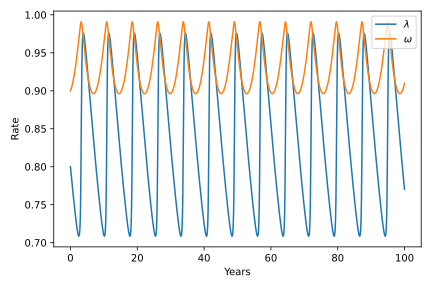
\includegraphics[scale=0.80]{goodwin.svg}
\includesvg[scale=0.75]{../imgs/goodwin.svg}
\end{center}
\end{frame}
%------------------------------------------------

\begin{frame}
% Equations will be in this format
\frametitle{Blocks of Highlighted Text}
\begin{block}{Block 1}
Lorem ipsum dolor sit amet, consectetur adipiscing elit. Integer lectus nisl, ultricies in feugiat rutrum, porttitor sit amet augue. Aliquam ut tortor mauris. Sed volutpat ante purus, quis accumsan dolor.
\end{block}

\begin{block}{Block 2}
Pellentesque sed tellus purus. Class aptent taciti sociosqu ad litora torquent per conubia nostra, per inceptos himenaeos. Vestibulum quis magna at risus dictum tempor eu vitae velit.
\end{block}

\begin{block}{Block 3}
Suspendisse tincidunt sagittis gravida. Curabitur condimentum, enim sed venenatis rutrum, ipsum neque consectetur orci, sed blandit justo nisi ac lacus.
\end{block}
\end{frame}

%------------------------------------------------

\begin{frame}
\frametitle{Multiple Columns}
\begin{columns}[c] % The "c" option specifies centered vertical alignment while the "t" option is used for top vertical alignment

\column{.45\textwidth} % Left column and width
\textbf{Heading}
\begin{enumerate}
\item Statement
\item Explanation
\item Example
\end{enumerate}

\column{.5\textwidth} % Right column and width
Lorem ipsum dolor sit amet, consectetur adipiscing elit. Integer lectus nisl, ultricies in feugiat rutrum, porttitor sit amet augue. Aliquam ut tortor mauris. Sed volutpat ante purus, quis accumsan dolor.

\end{columns}
\end{frame}

%------------------------------------------------
\section{Conclusion}
%------------------------------------------------

\begin{frame}
% Parameters will be in this format
\frametitle{Parameters}
\begin{table}
\begin{tabular}{l l l}
\toprule
\textbf{Treatments} & \textbf{Response 1} & \textbf{Response 2}\\
\midrule
Treatment 1 & 0.0003262 & 0.562 \\
Treatment 2 & 0.0015681 & 0.910 \\
Treatment 3 & 0.0009271 & 0.296 \\
\bottomrule
\end{tabular}
\caption{Table caption}
\end{table}
\end{frame}

%------------------------------------------------

\begin{frame}
\frametitle{Theorem}
\begin{theorem}[Mass--energy equivalence]
$E = mc^2$
\end{theorem}
\end{frame}

%------------------------------------------------

\begin{frame}[fragile] % Need to use the fragile option when verbatim is used in the slide
\frametitle{Verbatim}
\begin{example}[Theorem Slide Code]
\begin{verbatim}
\begin{frame}
\frametitle{Theorem}
\begin{theorem}[Mass--energy equivalence]
$E = mc^2$
\end{theorem}
\end{frame}\end{verbatim}
\end{example}
\end{frame}

%------------------------------------------------

\begin{frame}
\frametitle{Figure}
Uncomment the code on this slide to include your own image from the same directory as the template .TeX file.
%\begin{figure}
%\includegraphics[width=0.8\linewidth]{test}
%\end{figure}
\end{frame}

%------------------------------------------------

\begin{frame}[fragile] % Need to use the fragile option when verbatim is used in the slide
\frametitle{Citation}
An example of the \verb|\cite| command to cite within the presentation:\\~

This statement requires citation \cite{p1}.
\end{frame}

%------------------------------------------------
\begin{frame}[allowframebreaks]
\frametitle{References}
\footnotesize{
\begin{thebibliography}{99} % Beamer does not support BibTeX so references must be inserted manually as below
\begin{tiny}
\bibitem[Boldrin, 1990]{p1} Boldrin, Woodford (1990)
\newblock Equilibrium Models Displaying Endogenous Fluctuations and Chaos:  a Survey
\newblock \emph{Journal of Monetary Economics} 25(2), 189–222.

\bibitem[Ganti, 2019]{p1} Akhilesh Ganti (2019)
\newblock Exogenous Growth Definition
\newblock \emph{Investopedia}

\bibitem[Goodwin, 1982]{p1} Richard Goodwin (1982)
\newblock A Growth Cycle
\newblock \emph{Essays in Economic Dynamics} 165-170.

\bibitem[Grasseli, 2012]{p1} Grasseli, Lima, et al. (2012)
\newblock An Analysis of the Keen Model for Credit Expansion, Asset Price Bubbles and Financial Fragility
\newblock \emph{Mathematics and Financial Economics} 6(3), 191–210.

\bibitem[Keen, 1995]{p1} Steve Keen (1995)
\newblock Finance and Economic Breakdown:  Modeling Minsky’s “Financial Instability Hypothesis”
\newblock \emph{Journal of Post Keynesian Economics} 7(4), 607–635.

\bibitem[Maheswari, 2015]{p1} Aditya Maheshwari (2015)
\newblock An Empirical Study of Goodwin Growth Models
\newblock \emph{PhD Thesis}

\bibitem[Hunter, 2007]{p1} John Hunter (2007)
\newblock Matplotlib: A 2D Graphics Environment
\newblock \emph{Computing in Science and Engineering} 9(3), 90-95.

\bibitem[Minsky, 1992]{p1} Hyman Minsky (1992)
\newblock The Financial Instability Hypothesis
\newblock \emph{The Jerome Levy Economics Institue Working Paper} (74).

% Numpy
\bibitem[Harris, 2020]{p1} Harris, et al. (2020)
\newblock Array Programming with NumPy
\newblock \emph{Nature} 6, 357-362.

% Pandas
\bibitem[McKinney, 2010]{p1} Wes McKinney (2010)
\newblock Data Structures for Statistical Computing in Python

\bibitem[Rossum, 1995]{p1} Guido Rossum (1995)
\newblock Python Reference Manual
\newblock \emph{CWI}

% Scipy
\bibitem[Virtanen, 2020]{p1} Pauli Virtanen, et al. (2020)
\newblock SciPy 1.0: Fundamental Algorithms for Scientific Computing in Python
\newblock \emph{Nature Methods} 17, 261-272.

\bibitem[Weitzman, 1983]{p1} Martin Weitzman (1983)
\newblock Some  Macroeconomic  Implications  of  Alternative  Compensation Systems
\newblock \emph{The Economic Journal } 93(372), 763–783.

\end{tiny}
\end{thebibliography}
}
\end{frame}

%------------------------------------------------

\begin{frame}
\Huge{\centerline{Fin}}
\end{frame}

%----------------------------------------------------------------------------------------

\end{document} 